\documentclass{article}
\usepackage{amsmath}
\usepackage{tikz}
\usetikzlibrary{intersections}

\begin{document}

\begin{figure}[h]
    \centering
    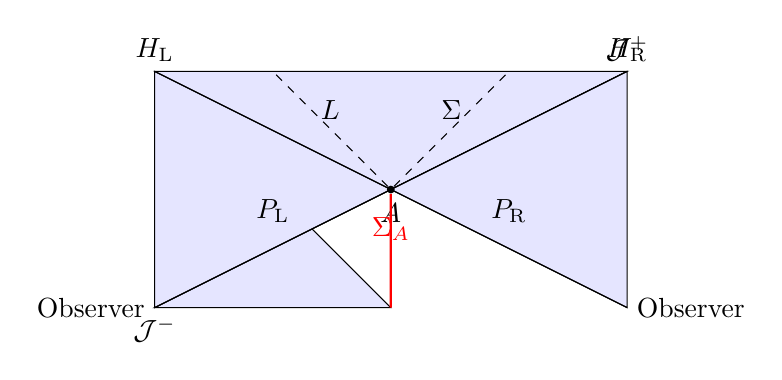
\begin{tikzpicture}[scale=1.5]
        % Define coordinates
        \coordinate (O) at (0,0);
        \coordinate (A) at (2,0);
        \coordinate (B) at (0,2);
        \coordinate (C) at (4,2);
        \coordinate (D) at (4,0);
        
        % Draw the square
        \draw[fill=blue!10] (O) -- (A) -- (B) -- (C) -- cycle;
        \draw[fill=blue!10] (O) -- (B) -- (D) -- (C) -- cycle;
        
        % Draw the diagonal lines
        \draw[name path=HL] (O) -- (C);
        \draw[name path=HR] (B) -- (D);
        
        % Draw the dashed line and the sphere
        \draw[dashed] (B) -- (C);
        \node[circle,fill,inner sep=1pt,label={below:$A$}] (A) at (2,1) {};
        
        % Draw the labels
        \node[left] at (O) {Observer};
        \node[right] at (D) {Observer};
        \node[above] at (C) {$\mathcal{J}^+$};
        \node[below] at (O) {$\mathcal{J}^-$};
        \node[above] at (B) {$H_{\rm L}$};
        \node[above] at (C) {$H_{\rm R}$};
        
        % Draw the red segment and the dotted line
        \draw[red,thick] (A) -- ++(0,-1) node[midway,above] {$\Sigma_A$};
        \draw[dotted,dashed] (A) -- ++(-1,1) node[midway,above] {$L$};
        \draw[dotted,dashed] (A) -- ++(1,1) node[midway,above] {$\Sigma$};
        
        % Label the static patches
        \node[below] at (1,1) {$P_{\rm L}$};
        \node[below] at (3,1) {$P_{\rm R}$};
    \end{tikzpicture}
    \caption{Two antipodal observers follow the antipodal trajectories defined by the left and right edge of the diagram. The diagonal lines form the cosmological horizons $H_{\rm L}$ and $H_{\rm R}$ for the two observers. They bound the two static patches $P_{\rm L}$ and $P_{\rm R}$ depicted in blue. The dashed line is an arbitrary global spacelike slice on which we place a sphere $A$ depicted by a black dot. $\Sigma_A\in\Sigma$ is the red segment and the future lightsheet emanating from $A$ is the dotted line.}
    \label{fig:cosmological_diagram}
\end{figure}

\end{document}